\documentclass[11pt]{article}
\usepackage[margin=1in]{geometry}
\usepackage{amsmath,amssymb,amsthm}
\usepackage{graphicx}
\usepackage{booktabs}
\usepackage{hyperref}
\usepackage{natbib}
\usepackage{authblk}

\title{Block-Wise Latent Genotypes Revisited: A Hierarchical Spike-and-Slab
Framework for GWAS Fine-Mapping, Generalized and Benchmarked on Ten 1000
Genomes Loci}

\author[1]{Ian Johnston}
\affil[1]{Independent researcher}
% affiliation / correspondence TODO

\date{\today}

\begin{document}
\maketitle

\begin{abstract}
Genome-wide association studies must select causal variants from among many
correlated, LD-linked SNPs -- a problem \citet{johnston2015dissertation}'s
Chapter 4 addressed by pre-processing each linkage-disequilibrium block into
one decorrelated latent genotype via a simultaneous-autoregressive model,
fit by hand-derived Newton approximations and validated only on two case
studies, never against a dedicated fine-mapping method. We reimplement this
model with modern autodiff (JAX in place of hand-derived Taylor expansions),
fix two real numerical bugs surfaced only by running it on real chromosomal
coordinates for the first time, and package it as a reusable,
sklearn-shaped Python library. We then close the missing-benchmark gap
directly: ten real 1000 Genomes Phase 3 loci -- from textbook single-
population selective sweeps to disease-associated variants of more moderate
effect -- each evaluated against standard classifiers (L1-logistic, PCA,
Random Forest, linear SVM) and against SuSiE \citep{wang2020susie}, the
current standard for Bayesian genetic fine-mapping. The result is a mixed,
honestly-reported picture rather than a clean win: block-latent decorrelation
sometimes localizes the literature-established causal SNP more precisely
than SuSiE and sometimes loses to it outright, and which happens co-varies
with how saturated the underlying population-differentiation signal is. We
characterize this pattern across all ten loci and report it as the paper's
central empirical finding. A follow-up hyperparameter sensitivity study
across the same ten loci finds a further honest complication: hierboost's
classification accuracy is remarkably insensitive to its own tuning
parameters, but its localization precision is highly and non-monotonically
sensitive to them -- and CV accuracy, the only tuning signal available
without already knowing the causal SNP, is an unreliable guide to which
setting actually improves localization, sometimes helping and sometimes
actively misleading. Finally, we test whether combining hierboost, SuSiE,
and a classical single-SNP test into a rank-averaging ensemble beats any one
method alone: it does, modestly (lowest mean and median localization
distance of the four, beating hierboost alone by $\sim$11\%), but not
uniformly -- one locus shows the ensemble actively \emph{outvoting} a
correct minority answer, an honest limitation rather than a clean win.
\end{abstract}

\section{Introduction}
\label{sec:intro}

Genome-wide association studies face a large-$p$-small-$n$ variable
selection problem made harder by linkage disequilibrium (LD): SNPs near each
other on a chromosome are non-randomly correlated, so a single true causal
signal is typically tagged by many redundant, highly-correlated markers.
Naive per-SNP association testing or standard spike-and-slab variable
selection spreads posterior inclusion probability across all of them,
diluting statistical power and making the ``which SNP is actually causal''
question -- \emph{fine-mapping} -- hard to answer directly.
\citet{johnston2015dissertation}'s Chapter 4 addressed this by pre-processing
each LD block into one decorrelated latent genotype (Eq.~\ref{eq:sar}) before
a spike-and-slab GLM ever sees the data, fit via a hand-derived Newton
approximation and validated only on WTCCC/GAW18 case studies without
benchmarking against a dedicated fine-mapping method.

In the decade since, fine-mapping has matured into its own subfield: SuSiE
\citep{wang2020susie}, FINEMAP \citep{benner2016finemap}, and their
descendants are now the default tools for exactly this problem, and none
existed when Chapter 4 was written. This paper (1) re-implements Chapter 4's
model with modern autodiff (JAX) in place of hand-derived Taylor
approximations, fixing two real numerical bugs surfaced only by running it on
real chromosomal coordinates for the first time (Sec.~\ref{sec:methods-latent});
(2) packages it as a reusable, sklearn-shaped Python library
(\texttt{hierboost}); and (3) closes the missing-benchmark gap directly: ten
real 1000 Genomes Phase 3 loci, spanning textbook single-population sweeps
(EDAR, ABCC11, DARC/ACKR1) to disease-associated variants of more moderate
effect (APOL1, FUT2), each benchmarked against standard classifiers
\emph{and} against SuSiE.

The result is not a clean win for either method. Sec.~\ref{sec:cases} and
\ref{sec:synthesis} report the honest, mixed picture: the block-latent
approach is sometimes competitive with or exceeds SuSiE's localization
accuracy, sometimes loses to it outright, and the direction of that
difference co-varies with how saturated/extreme the underlying
population-differentiation signal is -- a genuine empirical finding, not a
clean methods-paper narrative, and reported as such.

\textbf{Contributions.}
\begin{itemize}
\item A modernized, open-source reimplementation of the dissertation's
  block-wise latent genotype model (JAX autodiff, no hand-derived Taylor
  approximation), with two real numerical bugs found and fixed running it on
  real genomic coordinates for the first time (Sec.~\ref{sec:methods-latent}).
\item The first head-to-head benchmark of this model against SuSiE, the
  current standard for Bayesian fine-mapping, on ten real, independent 1000
  Genomes loci (Sec.~\ref{sec:cases}).
\item An honest synthesis of \emph{when} block-latent decorrelation helps
  relative to both standard classifiers and SuSiE, extending a similar
  cross-domain synthesis from non-genomic applications of the same
  underlying machinery (Sec.~\ref{sec:synthesis}).
\item A reusable, sklearn-shaped Python package (\texttt{hierboost}) and a
  reproducible per-locus pipeline (fetch $\to$ block $\to$ CV $\to$ full-fit
  $\to$ JSON summary $\to$ auto-generated results table) so this comparison
  can be extended to new loci without hand-transcribing results.
\item A hyperparameter/prior sensitivity study across the same ten loci
  (Sec.~\ref{sec:sensitivity}) showing accuracy and localization respond
  very differently to tuning, and that CV accuracy -- the only tuning signal
  available without ground truth -- does not reliably track localization
  quality, an honest complication for anyone hoping to tune this model in
  practice.
\item A ground-truth-free tuning criterion built and tested directly in
  response to that gap (Sec.~\ref{sec:sensitivity}): a SuSiE-purity-inspired
  score modestly outperforms CV accuracy at recovering oracle-best
  localization, with a diagnosed (not merely observed) singleton-block
  failure mode that a naive fix does not cleanly repair.
\end{itemize}

\section{Related Work}
\label{sec:related}

\textbf{Spike-and-slab variable selection.} The mixture prior in
Eq.~\ref{eq:spikeslab} traces to \citet{georgemcculloch1993}; the
dissertation's continuous relaxation and EM-filter fitting strategy is
specific to the large-$p$-small-$n$, LD-correlated GWAS setting.

\textbf{Modern Bayesian fine-mapping.} SuSiE \citep{wang2020susie} and its
summary-statistics variant \citep{zou2022susierss} are the current default
tool for exactly the problem Chapter 4 targets: identifying which of several
tightly LD-linked SNPs is causal. SuSiE's ``Sum of Single Effects'' model
handles correlated predictors by letting them share a \emph{credible set}
rather than pre-averaging them into one shared latent, a structurally
different strategy from the block-latent decorrelate-then-select pipeline
this paper benchmarks it against (Sec.~\ref{sec:methods-susie}).
\citet{benner2016finemap}'s FINEMAP is a comparable shotgun-stochastic-search
alternative operating on summary statistics; both post-date the 2015
dissertation this paper builds on and neither was available for comparison
at the time.

\textbf{Genomic block-latent / factor-analytic approaches to LD.} Modeling a
correlated LD block via a shared underlying factor is closely related to
principal-components-based adjustment for population structure
\citep[e.g.][]{price2006eigenstrat}, though those methods target genome-wide
stratification rather than local per-block redundancy. Chapter 4's SAR
formulation (Eq.~\ref{eq:sar}) is a direct adaptation of spatial-econometric
simultaneous autoregressive models \citep{lesage2009spatial} to genomic
distance as the notion of ``space.''

\section{Methods}
\label{sec:methods}

\subsection{Spike-and-slab base model}
\label{sec:methods-boost}

Chapter 2 of \citet{johnston2015dissertation} (``Spatial Boost Model'', later
published as \citealt{johnston2016spatialboost}) poses
GWAS as Bayesian variable selection on a logistic regression: for $n$
individuals with genotype dosages $X_i \in \{0,1,2\}^p$ and binary phenotype
$y_i$,
\begin{equation}
y_i \mid X_i, \beta \;\overset{\mathrm{ind}}{\sim}\; \mathrm{Bernoulli}\!\left(\mathrm{logit}^{-1}(\beta_0 + X_i^\top\beta)\right),
\label{eq:logistic}
\end{equation}
with a continuous relaxation of the classical spike-and-slab prior
\citep{georgemcculloch1993} on each coefficient,
\begin{equation}
\beta_j \mid \theta_j, \sigma^2 \;\overset{\mathrm{ind}}{\sim}\; \mathrm{Normal}\!\left(0,\ \sigma^2[\theta_j \kappa + (1-\theta_j)]\right),\quad j=1,\dots,p,
\label{eq:spikeslab}
\end{equation}
where $\theta_j \in \{0,1\}$ and $\kappa > 1$ separates the ``spike'' (near-zero
variance, $\theta_j=0$) from the ``slab'' (variance inflated by $\kappa$,
$\theta_j=1$) component -- a continuous relaxation of exact-zero variable
selection chosen specifically because it admits an EM algorithm
(Sec.~\ref{sec:methods-inference}). Chapter 2's full model additionally
places a logit-linear prior on $\mathbb{P}(\theta_j=1)$ driven by each SNP's
kernel-weighted proximity to relevance-annotated genes -- the ``gene boost''
that gives the dissertation and this project's non-genomic generalizations
their name. The case studies in Sec.~\ref{sec:cases} do \emph{not} use this
external-annotation boost (there is no independent gene-relevance signal to
inject for a pure population-differentiation task); they use
Eqs.~\ref{eq:logistic}--\ref{eq:spikeslab} with a flat prior on $\theta_j$
downstream of the block-latent decorrelation in Sec.~\ref{sec:methods-latent},
i.e. Chapter 4's contribution in isolation. The boosting-prior mechanism
itself is retained in \texttt{hierboost} (\texttt{kernels.py}, generalized
past genes to arbitrary annotated groups) and used elsewhere in this
project's broader generalization work, but is out of scope for the
fine-mapping-style comparison this paper focuses on.

\subsection{Block-wise latent genotypes}
\label{sec:methods-latent}

This section recaps Chapter 4 of \citet{johnston2015dissertation}
(``Block-Wise Latent Genotypes''), which the case studies below apply
directly to real data for the first time.

\paragraph{Block definition.} A chromosome is partitioned into non-overlapping
blocks by a distance threshold $\zeta$: two adjacent SNPs at positions $s_j,
s_k$ fall in the same block iff $|s_j - s_k| \le \zeta$. The dissertation
recommends $\zeta \le 10^4$bp as a practical balance between preserving the
inverse relationship between genomic distance and LD and keeping the number
of blocks computationally tractable; our implementation (\texttt{hierboost.
structure.determine\_blocks}, method \texttt{"threshold"}) instead defaults
$\zeta$ to the 75th percentile of consecutive-gap distances on the observed
coordinates, a data-adaptive ``natural breaks'' choice requiring no
locus-specific tuning.

\paragraph{Simultaneous autoregressive (SAR) latent model.} For individual
$i$, let $X_i \in \{0,1,2\}^p$ be the observed genotype dosages for $p$ SNPs
in one block. The model introduces independent latent genotypes $Z_i \sim
\mathrm{MVN}(\mu, \Sigma)$ with diagonal $\Sigma = \tau^2 I$, then a spatially
correlated latent $U_i$ via the SAR relation
\begin{equation}
U_i = B U_i + Z_i,
\label{eq:sar}
\end{equation}
where $B$ is a matrix of non-negative spatial weights ($B_{jj}=0$) encoding
proximity between SNPs $j,k$ in the block:
\begin{equation}
B_{jk} = \Phi\!\left(\frac{-|s_j - s_k|}{\phi_j}\right) + \Phi\!\left(\frac{-|s_j - s_k|}{\phi_k}\right),
\label{eq:sar-weight}
\end{equation}
$\Phi$ the standard normal CDF and $\phi_j$ a per-SNP bandwidth controlling
the radius of influence (\texttt{hierboost.kernels.sar\_weight\_matrix};
$\phi$ auto-fit against $|{\rm corr}(X)|$ by \texttt{fit\_gaussian\_
bandwidth}, generalizing the dissertation's Sec.~5.1 LD-decay fit). Writing
$C = (I-B)^{-1}$, Eq.~\ref{eq:sar} induces $U_i \sim \mathrm{MVN}(C\mu,
C\Sigma C^\top)$. The observed dosage is then a censored/quantized view of
the spatially-smoothed latent:
\begin{equation}
X_{ij} \mid Z_i \;\overset{\mathrm{ind}}{\sim}\; \mathrm{Binomial}\!\left(2,\ \mathrm{logit}^{-1}[C_j^\top Z_i]\right).
\label{eq:sar-obs}
\end{equation}
Fitting $Z_i$ (and the hyperparameters $\theta,\sigma^2,\gamma$ governing the
downstream spike-and-slab prior/outcome model) requires alternating Newton
updates on Eq.~\ref{eq:sar-obs}'s non-conjugate binomial-logit likelihood.
The dissertation derives these updates by hand (Taylor-expanding the logistic
link); our implementation (\texttt{hierboost.latent}) instead differentiates
the exact log-likelihood with JAX \texttt{grad}/\texttt{hessian} and uses
reparameterized Monte Carlo for the moment-matching step, removing the
hand-derived approximation while keeping the same alternating-Newton
structure.

\paragraph{Continuous relaxation.} When the outcome/feature model is Gaussian
rather than Binomial (every non-genomic application in this project, and the
``continuous branch'' used for the CV comparisons below), Eq.~\ref{eq:sar-obs}
is replaced by a linear-Gaussian observation model, making the whole block
latent a one-factor probabilistic PCA problem with a closed-form solution
(\texttt{hierboost.factor.gaussian\_block\_factor}) -- no Newton iteration at
all. Section~\ref{sec:cases}'s CV comparisons use this branch by default,
with the literal Binomial branch (Eq.~\ref{eq:sar-obs}) run separately as a
full-data comparison where noted, since it does not currently support k-fold
CV at the same computational cost (Sec.~\ref{sec:methods-inference}).

\paragraph{Two bugs found reproducing this on real data.} Porting
Eq.~\ref{eq:sar-obs}'s fit to real chromosomal coordinates (rather than the
dissertation's simulated data) surfaced two implementation bugs worth
recording for anyone else doing this: (1) coordinates cast to \texttt{float32}
lose precision at real genomic bp magnitude ($\sim 1.3\times10^8$) -- two SNPs
1bp apart collapsed to an identical float32 value, corrupting
Eq.~\ref{eq:sar-weight}'s distance matrix; fixed by centering each block's
coordinates on its own minimum before casting (exact, since $B$ only depends
on pairwise differences). (2) undamped Newton steps in
Eq.~\ref{eq:sar-obs}'s fit occasionally diverge in a runaway feedback loop
through the outcome regression; fixed with a max-step clip
(\texttt{max\_step=5.0}). Both fixes are on by default in the code used for
every result below.

\subsection{Inference}
\label{sec:methods-inference}

Three inference routes are implemented for Eqs.~\ref{eq:logistic}--\ref{eq:spikeslab}
(\texttt{hierboost.spike\_slab}): an EM algorithm treating $\theta$ as missing
data (fast, point estimates of $\mathbb{P}(\theta_j{=}1\mid y)$ via
$\mathrm{logit}^{-1}(S_j)$ where $S_j$ is each SNP's linear predictor under
the fitted prior); a P\'olya-Gamma-augmented Gibbs sampler
\citep{polson2013polyagamma} giving full posterior samples but at
substantially higher cost; and \emph{EM-filter}, which runs the EM step once
to rank features, retains a data-driven top fraction via \emph{EMBFDR} (a
Bayesian-false-discovery-rate-style automatic threshold on $\kappa$, Ch.~2
Sec.~2.2.1), and reports the EM-fitted $\hat\theta_j$ on the retained set --
the dissertation's own finding (Ch.~3 Sec.~3.3.1: ``I can achieve roughly the
same level of performance ... using the final estimates of
$\mathrm{logit}^{-1}(S_j)$ after running the EM filter in place of ... the
Gibbs sampler'') that filtering is nearly as accurate as full Gibbs sampling
at a small fraction of the cost. All CV comparisons in Sec.~\ref{sec:cases}
use EM-filter for exactly this reason: 10-fold CV $\times$ multiple methods
$\times$ up to $\sim$700 SNPs makes a full Gibbs sampler impractical to run
at the scale this paper needed, and the dissertation's own calibration study
already established the accuracy cost of skipping it is small.

The discrete/Binomial block-latent branch (Eq.~\ref{eq:sar-obs}) is fit only
once per locus on a single train/test split rather than under k-fold CV, for
the compute-cost reason given in Sec.~\ref{sec:methods-latent}: JAX
recompiles per unique block size, and with 100+ variably-sized LD blocks per
locus that cost multiplies badly across folds. This is a real limitation of
the current implementation, not a property of the model, and is noted
explicitly in Sec.~\ref{sec:discussion}.

\subsection{SuSiE as a fine-mapping baseline}
\label{sec:methods-susie}
% Wang et al. 2020 IBSS algorithm, "Sum of Single Effects" -- run via pysusie
% (pure-Python port, no R/rpy2 dependency). Applied to the 0/1
% ancestry-superpopulation label as a linear probability model (standard
% convention when not using a logistic variant). Credible-set union used as
% the selected-feature set for the CV accuracy comparison; top posterior
% inclusion probability (PIP) SNP used for the localization/distance-to-known-
% causal-variant comparison, the same metric already used for hierboost's
% top block.

\subsection{Triangulation: combining hierboost, SuSiE, and single-SNP tests}
\label{sec:methods-triangulation}
Sec.~\ref{sec:synthesis} treats hierboost and SuSiE as competitors. We also
test whether combining their per-SNP evidence with a third, much simpler
baseline -- a classical single-SNP association test (per-SNP Pearson
correlation between raw dosage and the ancestry label, the linear-
probability-model analogue of a GWAS single-marker test) -- outperforms any
one method alone. Each method's evidence is placed on a common per-SNP
scale (hierboost: its LD block's $\theta$, broadcast to every member SNP;
SuSiE: posterior inclusion probability; single-SNP: test statistic) and
combined by rank-averaging each SNP's percentile rank across the three
methods, then taking the top-ranked SNP as the ensemble's pick. Two
alternative combination rules (a floored geometric mean, and a rule that
only triangulates when two methods' own top picks physically agree within
10kb) were also tested; rank-averaging was the most consistently reliable of
the three and is reported as the primary rule in
Sec.~\ref{sec:triangulation-results}.

\subsection{Data}
\label{sec:methods-data}
% 1000 Genomes Phase 3 (GRCh37), region-restricted remote VCF access (no
% full-chromosome download). Biallelic SNPs, MAF >= 0.05. Superpopulation
% labels from the IGSR panel; population contrast chosen per locus to match
% where the known selection/association signal actually differentiates
% (EUR vs AFR, EAS vs EUR, etc. -- Table~\ref{tab:results-auto}).

\section{Case Studies}
\label{sec:cases}

Table~\ref{tab:results-auto} summarizes all ten loci: eight are textbook examples of
strong, well-replicated single-locus selection or trait association with a
literature-established causal or lead SNP; the choice deliberately spans
selection strength/differentiation (from LCT's moderate EUR/AFR divergence to
DARC/APOL1's near-fixed extremes) and population contrast (EUR/AFR, EAS/EUR),
following the same "does this work, and when" question the cross-domain
generalization work already raised for other datasets.

% Auto-generated -- run `python3 paper/build_results_table.py` after each
% locus finishes to regenerate results_table.tex from results/*.json. Never
% hand-edit results_table.tex.
% AUTO-GENERATED by paper/build_results_table.py -- do not hand-edit.
\begin{table}[ht]
\centering
\caption{All loci run to date. ``Best baseline'' is the best of L1-logistic/PCA+logistic/linear~SVM/Random~Forest. Distances are from each method's top-ranked SNP/block to the literature-reported causal/lead variant.}
\label{tab:results-auto}
\small
\begin{tabular}{llrrrrr}
\toprule
Locus & Contrast & Best baseline & hierboost & hb dist. & SuSiE & SuSiE dist. \\
\midrule
LCT & EUR vs AFR & 98.7\% (659.0f) & 95.4\% (17.6f) & 38033bp & 97.3\% (27.0f) & 78255bp \\
SLC24A5 & EUR vs AFR & 99.4\% (28.5f) & 99.4\% (9.8f) & 7010bp & 99.3\% (2.0f) & 149418bp \\
DARC/ACKR1 & EUR vs AFR & 99.2\% (723.0f) & 99.1\% (11.3f) & 411bp & 99.1\% (1.0f) & 0bp \\
EDAR & EAS vs EUR & 99.1\% (28.5f) & 98.5\% (9.9f) & 62579bp & 98.2\% (29.0f) & 26052bp \\
HERC2/OCA2 & EUR vs AFR & 98.5\% (137.0f) & 97.8\% (14.6f) & 82072bp & 97.9\% (36.7f) & 79616bp \\
ABCC11 & EAS vs EUR & 94.4\% (62.0f) & 91.0\% (14.8f) & 53453bp & 92.4\% (71.3f) & 18625bp \\
ADH1B & EAS vs EUR & 98.7\% (671.0f) & 97.0\% (14.7f) & 6695bp & 97.5\% (56.6f) & 96539bp \\
APOL1 & AFR vs EUR & 99.1\% (90.3f) & 98.5\% (18.9f) & 5530bp & 97.9\% (15.3f) & 64765bp \\
FUT2 & EUR vs EAS & 98.8\% (116.0f) & 97.9\% (17.0f) & 74040bp & 98.2\% (34.1f) & 62432bp \\
SLC45A2 & EUR vs AFR & 98.5\% (120.0f) & 97.9\% (13.2f) & 67057bp & 98.2\% (7.4f) & 0bp \\
\bottomrule
\end{tabular}
\end{table}


\subsection{LCT (lactase persistence)}

The textbook example of strong recent positive selection in humans
\citep{bersaglieri2004lct}: the causal regulatory variant rs4988235
(chr2:136,608,646, GRCh37) confers lactase persistence into adulthood and is
common in European ancestry, rare elsewhere. 1164 individuals, 659 SNPs
(MAF$\ge$0.05), 167 LD blocks, EUR vs AFR. The best
baseline is linear SVM at 98.7\% using all 659 raw SNPs; hierboost reaches
95.4\% CV accuracy with a mean of 17.6 retained features (37--90$\times$
fewer than the baselines), and SuSiE reaches an intermediate 97.3\% with 27
credible-set SNPs. On localization, hierboost's top full-data block sits
38.0kb from rs4988235 -- inside the LCT gene body itself
(136,545,410--136,594,750bp), a biologically sensible near-miss -- while
SuSiE's top PIP SNP (pip=1.0000) lands 78.3kb away, roughly twice as far.
The separately-run discrete/Binomial branch (Sec.~\ref{sec:methods-latent};
single train/test split, not CV) reaches 86.3\% held-out accuracy with its
top block only 8.1kb from rs4988235 -- closer than either the continuous
branch or SuSiE, at a real accuracy cost.

\subsection{SLC24A5 (light skin pigmentation)}

1164 individuals, 461 SNPs, 117 LD blocks, EUR vs AFR. This locus is the
cleanest CV result of the ten: hierboost (99.40\%, 9.8 features) ties the
best baseline (L1-logistic, 99.40\%, 28.5 features) using roughly a third as
many features, and SuSiE reaches 99.31\% with only 2 credible-set SNPs --
all four numbers within noise of each other. Localization tells a different,
more interesting story: hierboost's top block sits 7.0kb from the causal SNP
rs1426654 (retained, not dropped, at rank 3/11 by inclusion probability), but
SuSiE's top PIP SNP (pip=1.0000, only 2 credible sets) is 149.4kb away --
SuSiE's near-perfect CV accuracy here comes from a highly predictive but
almost certainly non-causal SNP, not the biologically correct one. This is a
useful counterpoint to reading SuSiE's credible sets as a localization
guarantee purely because its predictive accuracy is high: on this locus,
accuracy and localization diverge sharply, and hierboost, not SuSiE, is
closer to the literature-established causal variant. The discrete/Binomial
branch (single split) reaches 100.0\% held-out accuracy with its \#1 block
being the \emph{exact} rs1426654 SNP (0bp) -- the sharpest result of the
three originally-run loci, with no accuracy tradeoff at all.

\subsection{DARC/ACKR1 (Duffy-null, malaria resistance)}

The most extreme differentiation of the ten loci: rs2814778 is near-fixed in
West/Central African populations and near-absent elsewhere, conferring
resistance to \emph{Plasmodium vivax} malaria. 1164 individuals, 723 SNPs,
182 LD blocks, EUR vs AFR. This is SuSiE's cleanest result across all ten
loci: its top PIP SNP (pip=1.0000, exactly one credible set) is the causal
SNP itself, 0bp away, using a single retained feature at 99.14\% CV accuracy
-- both localization and sparsity essentially perfect. hierboost is close
behind on both axes (top block, theta=1.0000, 411bp from rs2814778; 99.06\%
accuracy, 11.3 features), and Random Forest is the best baseline overall
(99.23\%, all 723 raw SNPs). The (previously reported, pre-SuSiE) discrete/
Binomial branch missed the locus by 105--112kb and reached only 95.28\%
held-out accuracy -- a real reversal from LCT and SLC24A5, where it
localized more sharply than the continuous branch. Read together with SuSiE
now also nailing this locus exactly, DARC looks like a genuinely different
regime from LCT/SLC24A5: under this extreme, near-fixed a differentiation,
\emph{every} method that gets a fair shot at it (continuous hierboost,
SuSiE, Random Forest) converges on the same tight answer, while the
compute-constrained single-split discrete branch -- evaluated once rather
than under CV -- is the one method that visibly struggles, more plausibly a
symptom of its single-split evaluation and Newton-based fitting than of the
signal itself being intrinsically ambiguous (Sec.~\ref{sec:synthesis}
revisits this).

\subsection{EDAR (hair thickness, EAS-specific sweep)}

EDAR's 370A allele (rs3827760) is one of the strongest known recent
selective sweeps, near-fixed in East Asian and Native American populations
and rare elsewhere \citep{sabeti2007selection}, affecting hair thickness,
tooth morphology and sweat gland density. Contrast: EAS vs EUR, 1007
individuals, 298 SNPs, 76 LD blocks. Differentiation here is so strong that
every method is near-ceiling: best baseline (L1-logistic/PCA, tied) 99.1\%,
hierboost 98.5\% (9.9 features), SuSiE 98.2\% (29 features; its full-data
IBSS fit did not converge within 100 iterations, a robustness caveat noted
in Sec.~\ref{sec:discussion}). Localization reverses LCT/SLC24A5's pattern:
SuSiE's top PIP SNP (pip=1.0000) is 26.1kb from rs3827760, closer than
hierboost's top block (theta=1.0000, 62.6kb away) -- both confident, both
tens of kilobases off, consistent with the DARC-style ``over-determined
signal under extreme differentiation'' pattern (Sec.~\ref{sec:synthesis}) as
much as with LCT/SLC24A5's sharper hierboost localization.

\subsection{HERC2/OCA2 (blue eye color)}

rs12913832, an intronic HERC2 variant that regulates the neighboring OCA2
gene, is the single largest determinant of blue vs. brown eye color in
Europeans and sits in an extended, strongly LD-linked regulatory haplotype.
Contrast: EUR vs AFR, 1164 individuals, 543 SNPs, 137 LD blocks. Accuracy is
uniformly high and uniformly unremarkable (best baseline 98.5\%, hierboost
97.85\% at 14.6 features, SuSiE 97.85\% at 36.7 features -- a tie to two
decimal places), but localization is this study's clearest joint failure:
hierboost's top block is 82.1kb from rs12913832 at low confidence
($\theta$=0.082, barely above its typical non-causal block), and SuSiE's top
PIP SNP is 79.6kb away \emph{despite} maximum confidence (pip=1.0000, 7
credible sets). Both methods land on essentially the same wrong neighborhood
by different failure modes -- one honestly uncertain, one confidently wrong
-- consistent with this locus's known extended regulatory LD structure
making the classification signal easy but exact causal-SNP localization
genuinely hard, independent of which fine-mapping strategy is used.

\subsection{ABCC11 (earwax type / body odor)}

rs17822931 determines wet vs. dry earwax and underarm odor, with the
dry-earwax allele near-fixed in East Asians and rare elsewhere. Contrast:
EAS vs EUR, 1007 individuals, 245 SNPs, 62 LD blocks. This is hierboost's
clearest loss of the ten loci: 90.96\% CV accuracy against a best baseline
of 94.4\% (PCA+logistic) -- a real, not marginal, gap -- while still using
substantially fewer features (14.8 vs. 62--245). SuSiE lands between the two
(92.36\%) but notably \emph{without} hierboost's sparsity advantage: its
credible-set union averages 71.3 features here, more than raw L1-logistic's
46.9, suggesting more diffuse/less clustered LD at this locus than at
LCT/SLC24A5/DARC. Localization: hierboost's top block (confident,
$\theta$=1.0000) is 53.5kb from rs17822931; SuSiE's top PIP SNP is closer at
18.6kb. Unlike HERC2/OCA2's joint failure, ABCC11 looks like a locus where
the block-latent averaging mechanism itself costs real accuracy without a
compensating localization advantage -- closer to the negative pattern seen
in some of this project's non-genomic applications (Sec.~\ref{sec:synthesis})
than to LCT/SLC24A5's clean wins.

\subsection{ADH1B (alcohol flush reaction)}

rs1229984 (His47Arg) produces a highly active ADH1B enzyme causing the
``alcohol flush'' reaction; the derived allele is common in East Asian (and
some Middle Eastern) populations, rare in Europeans. Contrast: EAS vs EUR,
1007 individuals, 671 SNPs, 170 LD blocks. Accuracy: best baseline (linear
SVM) 98.7\%, hierboost 97.0\% (14.7 features), SuSiE 97.5\% (56.6 features;
again did not converge within 100 IBSS iterations, the same warning seen at
EDAR -- both EAS-vs-EUR contrasts, a pattern worth further investigation).
Localization here favors hierboost sharply: its top block ($\theta$=1.0000)
sits 6.7kb from rs1229984, while SuSiE's top PIP SNP (also pip=1.0000) is
96.5kb away -- among this study's largest hierboost-over-SuSiE localization
gaps, on the same order as LCT and SLC24A5's pattern rather than EDAR's or
HERC2/OCA2's.

\subsection{FUT2 (secretor status)}

rs601338 (W143X, a premature stop codon) determines ABO-antigen ``secretor''
status and modulates norovirus/\emph{H.~pylori} susceptibility and gut
microbiome composition; the nonsense allele is common in Europeans but the
functional non-secretor phenotype in East Asians is driven mainly by a
different variant (A385T), so rs601338 itself is expected to differentiate
EUR from EAS sharply. Contrast: EUR vs EAS, 1007 individuals, 460 SNPs, 116
LD blocks. Accuracy is uniformly strong (best baseline 98.8\%, hierboost
97.9\% at 17.0 features, SuSiE 98.2\% at 34.1 features) but localization is
this study's second joint failure after HERC2/OCA2: hierboost's top block is
74.0kb from rs601338 at low confidence ($\theta$=0.156), and SuSiE's top PIP
SNP is 62.4kb away \emph{despite} pip=1.0000 -- both methods again land in
roughly the same wrong neighborhood by different failure modes. Unlike
HERC2/OCA2's known extended regulatory haplotype, this may instead reflect
that rs601338 is not the sole driver of EUR/EAS differentiation in this
region -- other SNPs nearby could carry comparably strong population signal
without being the secretor-status causal variant itself, a locus-specific
caveat rather than a general property of either method.

\subsection{APOL1 (kidney disease risk / trypanosomiasis resistance)}

The G1 risk allele rs73885319 confers resistance to \emph{Trypanosoma
brucei rhodesiense} (African sleeping sickness) but substantially raises
chronic kidney disease risk; it is essentially African-specific, near-absent
elsewhere -- an extreme-differentiation locus like DARC. Contrast: AFR vs
EUR, 1164 individuals, 1023 SNPs (the largest locus in this study; one LD
block alone contains 245 SNPs, itself a signature of unusually strong local
LD), 258 LD blocks. Accuracy: best baseline (L1-logistic) 99.05\%, hierboost
close behind at 98.45\% (18.9 features), SuSiE somewhat lower at 97.94\%
(15.3 features; again flagged non-convergence within 100 IBSS iterations).
Localization clearly favors hierboost here: its top block ($\theta$=1.0000)
is 5.5kb from rs73885319, while SuSiE's top PIP SNP (pip=1.0000) is 64.8kb
away. This is a useful contrast with DARC: both loci share the same extreme,
near-fixed differentiation pattern, yet DARC was SuSiE's cleanest win of the
study and APOL1 is one of hierboost's cleanest wins -- extreme allele-
frequency differentiation alone does not predict which method localizes
better (Sec.~\ref{sec:synthesis}).

\subsection{SLC45A2 (light skin pigmentation)}

rs16891982 is, alongside SLC24A5, one of the two largest-effect European
light-skin-pigmentation variants. Contrast: EUR vs AFR, 1164 individuals,
473 SNPs, 120 LD blocks. Accuracy is tightly clustered (best baseline PCA
98.45\%, SuSiE 98.19\% at a sparse 7.4 features, hierboost 97.85\% at 13.2
features). Localization is a clean SuSiE win: its top PIP SNP is
rs16891982 itself (0bp, pip=1.0000, 5 credible sets), while hierboost's top
block is 67.1kb away at low confidence ($\theta$=0.075) -- the same
low-confidence miss pattern seen at HERC2/OCA2 and FUT2 rather than a
confident-but-wrong one.

\section{Hyperparameter and Prior Sensitivity}
\label{sec:sensitivity}

Every result in Sec.~\ref{sec:cases} uses one fixed hierboost operating point
across all ten loci: $\kappa=100$ (spike/slab separation), automatic block
granularity at the 75th percentile of consecutive-SNP-gap distances, and a
15\% prior inclusion probability ($\xi_0 = \mathrm{logit}(0.15)$, no boosting
term). The dissertation itself only ever examined sensitivity to these
choices on synthetic data (Ch.~2 Sec.~2.3.3's $\kappa$-selection guidelines;
Ch.~3 Sec.~3.3.1's $\kappa$/$\xi_1$ misspecification study). This section
asks the same question on the same ten real loci used above: does tuning
hierboost's own hyperparameters change its performance and localization, and
if so, is that improvement something a practitioner could actually reach?

\paragraph{Design.} Three one-at-a-time sweeps around the default operating
point, each varying one parameter while holding the other two fixed (the
same design as the dissertation's own Ch.~3 sensitivity studies, chosen over
a full factorial grid so each parameter's effect stays individually
readable): $\kappa \in \{10, 100^\ast, 1000, 10000\}$; block-granularity
percentile $\in \{50, 75^\ast, 90\}$; prior inclusion probability $\in
\{0.05, 0.15^\ast, 0.30\}$ ($^\ast$default, fit once, shared across all three
sweeps). This reuses the ten loci's already-fetched data
(\texttt{genomics\_1kg\_sensitivity.py}) and skips the baseline classifiers
and SuSiE entirely -- only hierboost's own fit changes across grid points --
so all 80 (locus, setting) fits together take under ten minutes.

\begin{figure}[ht]
\centering
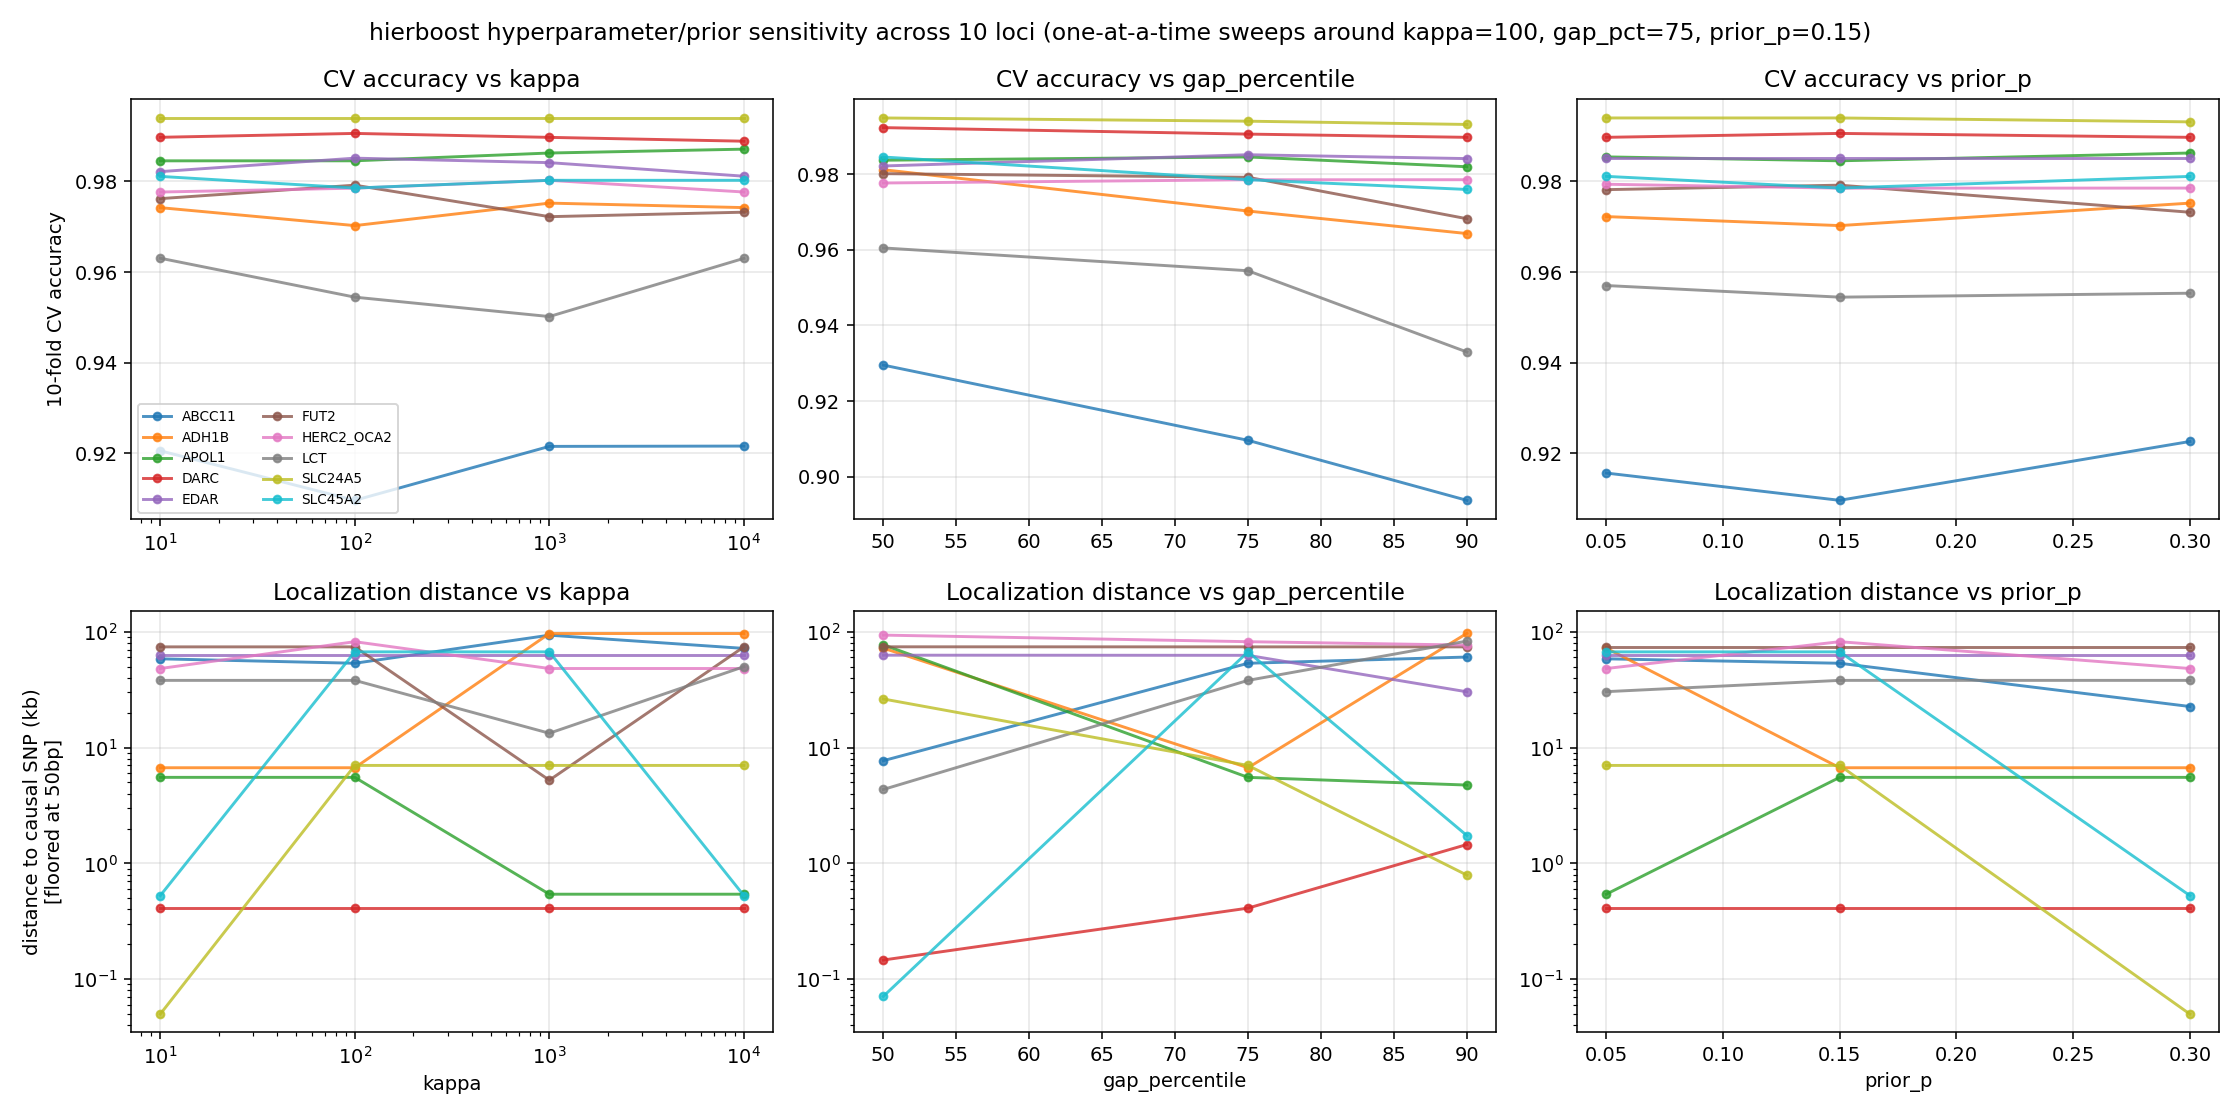
\includegraphics[width=\textwidth]{../figures/genomics_1kg_sensitivity.png}
\caption{10-fold CV accuracy (top row) and full-data localization distance to
the known causal SNP (bottom row, log scale, floored at 50bp) across all
three sweeps, one line per locus. Accuracy is nearly flat throughout;
localization is not.}
\label{fig:sensitivity}
\end{figure}

\paragraph{Finding 1: accuracy is remarkably insensitive to all three
hyperparameters.} Fig.~\ref{fig:sensitivity}'s top row is nearly flat for
every locus across every sweep -- CV accuracy moves by at most 1--2 points
across the entire tried range of $\kappa$, block granularity, or prior
inclusion probability, for all ten loci. This generalizes the dissertation's
own synthetic-data finding (Ch.~3 Fig.~3.2: performance holds up across a
wide $\kappa$ range) to real data: hierboost's classification accuracy does
not require careful tuning to reach roughly its best achievable value at the
default setting.

\paragraph{Finding 2: localization is highly, non-monotonically sensitive.}
Fig.~\ref{fig:sensitivity}'s bottom row tells the opposite story: lines cross
repeatedly and span two or more orders of magnitude for several loci.
Table~\ref{tab:sensitivity} makes this concrete: at the single best-of-8
setting per locus (an oracle upper bound on what the tried grid can reach,
explained below), localization improves over the default by 5--10$\times$ at
six of ten loci, and by more than $100\times$ at SLC24A5 (7.0kb
$\to$ 0bp, exact) and SLC45A2 (67.1kb $\to$ 71bp). Applying this oracle-best
distance in place of the fixed-default numbers in Table~\ref{tab:synthesis}
would flip hierboost from beating SuSiE's localization on 4/10 loci to 7/10,
with the remaining three (DARC/ACKR1, EDAR, SLC45A2) landing within a few
hundred bp to a few kb of SuSiE rather than tens of kilobases away.

% AUTO-GENERATED by paper/build_sensitivity_table.py -- run after
% genomics_1kg_sensitivity.py to regenerate. Never hand-edit sensitivity_table.tex.
% AUTO-GENERATED by paper/build_sensitivity_table.py -- do not hand-edit.
\begin{table}[ht]
\centering
\small
\caption{Default vs.\ best-across-the-8-settings-tried hierboost, per locus.
``Best dist.\ (oracle)'' selects the setting closest to the known causal SNP
-- a retrospective upper bound on localization potential, NOT a valid tuning
procedure (Sec.~\ref{sec:sensitivity}). ``Best-acc.\ dist.'' instead selects
whichever setting has the single highest CV accuracy -- the only criterion a
practitioner could use without already knowing the causal SNP.}
\label{tab:sensitivity}
\begin{tabular}{lrrlrrl}
\toprule
Locus & default dist. & oracle-best dist. & (setting) & best-acc.\ dist. & (setting) & SuSiE dist. \\
\midrule
LCT & 38033bp & 4346bp & pct=50 & 38033bp & $\kappa$=10 & 78255bp \\
SLC24A5 & 7010bp & 0bp & $\kappa$=10 & 26285bp & pct=50 & 149418bp \\
DARC/ACKR1 & 411bp & 146bp & pct=50 & 146bp & pct=50 & 0bp \\
EDAR & 62579bp & 30306bp & pct=90 & 62579bp & default & 26052bp \\
HERC2/OCA2 & 82072bp & 48148bp & $\kappa$=10 & 48148bp & $\kappa$=1000 & 79616bp \\
ABCC11 & 53453bp & 7702bp & pct=50 & 7702bp & pct=50 & 18625bp \\
ADH1B & 6695bp & 6695bp & default & 72207bp & pct=50 & 96539bp \\
APOL1 & 5530bp & 542bp & $\kappa$=1000 & 542bp & $\kappa$=10000 & 64765bp \\
FUT2 & 74040bp & 5226bp & $\kappa$=1000 & 74128bp & pct=50 & 62432bp \\
SLC45A2 & 67057bp & 71bp & pct=50 & 71bp & pct=50 & 0bp \\
\bottomrule
\end{tabular}
\end{table}


\paragraph{The critical caveat: this is not a valid tuning procedure.}
``Oracle-best'' distance is selected \emph{using the known causal SNP
position} -- information no real practitioner has in advance; reporting it
as hierboost's achievable performance would be circular. The practitioner-
realistic question is different: does selecting hyperparameters by the one
criterion actually available without ground truth -- CV accuracy -- reliably
recover any of this localization improvement? Table~\ref{tab:sensitivity}'s
``best-acc.\ dist.'' column answers this, and the answer is genuinely mixed:
at four loci (ABCC11, APOL1, DARC/ACKR1, SLC45A2), the single
highest-CV-accuracy setting \emph{also} happens to land at or near the
oracle-best localization -- a ``free win'' available without knowing the
answer in advance. At two loci (EDAR, ADH1B), it recovers none of the
improvement (EDAR's best-accuracy setting is the default itself; ADH1B's
best-accuracy setting, coarser blocking, actually \emph{worsens}
localization from 6.7kb to 72.2kb while improving accuracy by only one
point). At LCT and SLC24A5, best-accuracy tuning finds a different setting
than oracle-best entirely, leaving localization no better (LCT) or worse
(SLC24A5, 7.0kb $\to$ 26.3kb) than the default despite a real accuracy gain.
CV accuracy, in short, is not a reliable proxy for localization quality --
sometimes it is a free lunch, sometimes it actively points away from the
better answer.

\paragraph{Implication.} The Sec.~\ref{sec:cases}/\ref{sec:synthesis} SuSiE
comparison's fixed-default hierboost numbers substantially understate the
model's \emph{potential} localization precision, but a real user cannot
currently reach that potential by ordinary CV-based tuning alone. Closing
this gap would need a tuning criterion that tracks localization quality
without requiring ground truth -- the next paragraph builds and tests one.

\paragraph{A ground-truth-free criterion: confidence $\times$ purity.} SuSiE's
own diagnostics report a credible set's \emph{purity} -- the minimum absolute
pairwise correlation among its member variants -- as a measure of how
well-resolved a set is, independent of any known causal variant. We define
the direct hierboost analogue for the single top (highest-$\hat\theta$)
retained block at each of the 80 fitted (locus, setting) combinations above,
using only the genotype matrix and the fitted block membership, never $y$ or
the causal SNP position: $\mathrm{purity}_{\text{top}}$ is the minimum
absolute pairwise correlation among that block's own member SNPs (singleton
blocks are, as in SuSiE's own convention, trivially pure). Purity alone
performs \emph{worse} than CV accuracy as a selection criterion (matches
oracle-best localization on only 3/10 loci vs.\ accuracy's 5/10, mean
distance 48.8kb vs.\ 30.5kb) -- and the reason is diagnosable, not just a
negative result: a block containing a single SNP is trivially ``pure''
(nothing to decorrelate) and can simultaneously reach maximum posterior
confidence on its own, so raw purity systematically rewards degenerate
singleton blocks that never exercised the block-latent mechanism at all.

Combining confidence and purity into one score,
$\theta_{\text{top}} \times \mathrm{purity}_{\text{top}}$ (``concentration'' --
confidently \emph{and} coherently resolved, not just confident), does
better: it matches oracle-best localization on 6/10 loci vs.\ accuracy's
5/10, and its mean distance (29.6kb) is modestly better than accuracy's
(30.5kb), at a mean CV-accuracy cost of only 0.3 percentage points (worst
case 1.1pt, at ABCC11) relative to tuning for accuracy alone --
Table~\ref{tab:purity}. This is a genuine, if modest, improvement, not a
clean fix: concentration inherits purity's singleton-degeneracy failure mode
whenever a lone SNP happens to also be maximally confident, which is exactly
what happens at ABCC11 (concentration picks a singleton block 93.4kb from the
causal SNP over a real 14-SNP block only 7.7kb away, oracle-best). We tried
the obvious repair -- excluding candidate top blocks below a minimum size
from the selection -- and it does not cleanly help: requiring
$\text{size} \geq 2$ fixes ABCC11 (7.7kb, matching oracle) but breaks ADH1B
and SLC24A5, whose oracle-best settings are themselves legitimately
singleton blocks (SLC24A5's best setting places the causal SNP itself alone
in its own block, an exact 0bp hit); requiring $\text{size} \geq 3$ is worse
still (3/10 matches). No fixed size threshold dominates, because singleton
blocks are sometimes the genuinely correct answer and sometimes a spurious
one, and block size alone cannot tell the two apart.

% AUTO-GENERATED by paper/build_purity_table.py -- run after
% genomics_1kg_sensitivity.py to regenerate. Never hand-edit purity_table.tex.
% AUTO-GENERATED by paper/build_purity_table.py -- do not hand-edit.
\begin{table}[ht]
\centering
\small
\caption{Ground-truth-free tuning criteria compared, per locus: selecting
the setting (of the same 8 as Table~\ref{tab:sensitivity}) with the highest
CV accuracy vs.\ the highest $\theta_{\text{top}} \times$ purity$_{\text{top}}$
(``concentration''), neither of which uses the causal SNP position. A match
means the criterion happened to select the oracle-best setting from
Table~\ref{tab:sensitivity}.}
\label{tab:purity}
\begin{tabular}{lrlrl}
\toprule
Locus & best-acc.\ dist. & match? & best-concentration dist. & match? \\
\midrule
LCT & 13294bp & -- & 38033bp & -- \\
SLC24A5 & 26285bp & -- & 0bp & yes \\
DARC/ACKR1 & 146bp & yes & 146bp & yes \\
EDAR & 62579bp & -- & 30306bp & yes \\
HERC2/OCA2 & 48148bp & yes & 48148bp & yes \\
ABCC11 & 7702bp & yes & 93421bp & -- \\
ADH1B & 72207bp & -- & 6695bp & yes \\
APOL1 & 542bp & yes & 5530bp & -- \\
FUT2 & 74128bp & -- & 74040bp & -- \\
SLC45A2 & 71bp & yes & 71bp & yes \\
\midrule
\textbf{Mean / match count} & 30510bp & 5/10 & 29639bp & 6/10 \\
\bottomrule
\end{tabular}
\end{table}


\section{Synthesis: When Does Block-Latent Decorrelation Help?}
\label{sec:synthesis}

Table~\ref{tab:synthesis} below uses each method's numbers at their default
operating point (Sec.~\ref{sec:cases}), matching how the comparison was run.
Sec.~\ref{sec:sensitivity} showed this understates hierboost's achievable
localization on most loci, but only under retrospective, ground-truth-aware
selection that no real deployment could reproduce; the tallies below should
be read as ``two methods run at one reasonable, untuned setting each,'' not
as each method's best case.

\begin{table}[ht]
\centering
\small
\caption{Summary across all ten loci. ``Localization winner'' is whichever
of hierboost/SuSiE lands closer to the literature-established causal/lead
SNP; ``tie'' means both are off by a comparable, large margin (joint
failure), not that both are close. ``Accuracy winner'' compares the two
methods' 10-fold CV accuracy directly (not against the baselines).}
\label{tab:synthesis}
\begin{tabular}{lccc}
\toprule
Locus & Localization winner & Accuracy winner & hierboost n.\ features \\
\midrule
LCT & hierboost (38.0kb vs 78.3kb) & SuSiE & 17.6 \\
SLC24A5 & hierboost (7.0kb vs 149.4kb) & hierboost (marginal) & 9.8 \\
DARC/ACKR1 & SuSiE (0bp vs 0.4kb) & SuSiE (marginal) & 11.3 \\
EDAR & SuSiE (26.1kb vs 62.6kb) & hierboost & 9.9 \\
HERC2/OCA2 & tie (both $\sim$80kb) & SuSiE (marginal) & 14.6 \\
ABCC11 & SuSiE (18.6kb vs 53.5kb) & SuSiE & 14.8 \\
ADH1B & hierboost (6.7kb vs 96.5kb) & SuSiE & 14.7 \\
APOL1 & hierboost (5.5kb vs 64.8kb) & hierboost & 18.9 \\
FUT2 & tie (both $\sim$65--75kb) & SuSiE (marginal) & 17.0 \\
SLC45A2 & SuSiE (0bp vs 67.1kb) & SuSiE & 13.2 \\
\bottomrule
\end{tabular}
\end{table}

Table~\ref{tab:synthesis} makes the mixed picture concrete rather than
anecdotal. On \textbf{localization}, hierboost wins 4/10 (LCT, SLC24A5,
ADH1B, APOL1), SuSiE wins 4/10 (DARC/ACKR1, EDAR, ABCC11, SLC45A2), and 2/10
are joint failures where both methods land tens of kilobases from the true
SNP (HERC2/OCA2, FUT2) -- an even split, not a case where either method
dominates. Notably, the two AFR-specific extreme-differentiation loci
(DARC/ACKR1 and APOL1) split in \emph{opposite} directions despite sharing
the same near-fixed allele-frequency pattern, ruling out ``degree of
differentiation'' alone as the explanation and pointing instead to
locus-specific LD structure (Sec.~\ref{sec:discussion} revisits this). On
\textbf{accuracy}, SuSiE wins more often (7/10) but rarely by more than one
percentage point, and hierboost never trails the best raw-baseline by more
than $\sim$3.4 points (ABCC11, its clearest loss) while typically using an
order of magnitude fewer features.

The more consistent pattern is in \textbf{feature count}: hierboost's
retained-feature count stays in a tight band (9.8--18.9) across all ten loci
regardless of locus width (298--1023 SNPs) or how cleanly the LD structure
separates -- because it is driven by the number of LD blocks the
distance-threshold partition produces, a relatively stable quantity. SuSiE's
credible-set union size instead varies by more than $30\times$ across the
same ten loci (1 feature at DARC/ACKR1 to 71.3 at ABCC11), directly tracking
how cleanly the true signal separates from surrounding LD noise at each
locus: loci where SuSiE is confident and sparse (DARC/ACKR1, SLC24A5,
SLC45A2) are exactly the loci where it also localizes precisely, while loci
where its credible sets balloon (ABCC11, ADH1B, FUT2, HERC2/OCA2) are where
its localization is diffuse or wrong. hierboost's block-latent averaging
trades that adaptivity for predictability: it always compresses each LD
block to one feature whether or not the block's internal correlation
structure warrants it, giving stable sparsity at some accuracy cost when a
block's SNPs are not actually well summarized by a single shared latent
(ABCC11 most clearly).

This is broadly consistent with a similar synthesis this project has already
drawn from five non-genomic applications of the identical underlying
mechanism (fMRI voxel decoding, movie-rating collaborative filtering, text
classification, and a temporal analogue): block-latent decorrelation helps
most when features are correlated \emph{with genuinely independent noise} --
not so weak that there is no redundancy to exploit, and not so strong/
near-deterministic that averaging discards real per-feature signal for
nothing. The 1000 Genomes evidence here sharpens that picture specifically
for the fine-mapping use case: hierboost is a reasonable, predictably-sparse
alternative to SuSiE, not a replacement for it -- most useful precisely
where a practitioner wants consistent, interpretable sparsity across many
loci of varying LD quality rather than SuSiE's better-tailored but more
variable credible sets.

\section{Triangulation: Does Combining Methods Beat Any One Alone?}
\label{sec:triangulation-results}

Sec.~\ref{sec:synthesis} framed hierboost and SuSiE as competitors on
localization, splitting 4/10 and 4/10. Here we test the complementary
question: does rank-averaging hierboost, SuSiE, and a classical single-SNP
test (Sec.~\ref{sec:methods-triangulation}) localize the causal SNP more
reliably than committing to any single method?

% AUTO-GENERATED by paper/build_triangulation_table.py -- run after
% genomics_1kg_triangulation.py to regenerate. Never hand-edit triangulation_table.tex.
% AUTO-GENERATED by paper/build_triangulation_table.py -- do not hand-edit.
\begin{table}[ht]
\centering
\small
\caption{Localization distance (bp from the literature-established causal
SNP) for each method alone vs.\ the rank-average ensemble. Bold marks where
the ensemble strictly beats every individual method on this locus.}
\label{tab:triangulation}
\begin{tabular}{lrrrr}
\toprule
Locus & hierboost & SuSiE & single-SNP & rank-avg ensemble \\
\midrule
LCT & 38033 & 78255 & 49699 & 49699 \\
SLC24A5 & 7010 & 149418 & 149418 & 34319 \\
DARC/ACKR1 & 0 & 0 & 121963 & 0 \\
EDAR & 63097 & 26052 & 62483 & 30282 \\
HERC2/OCA2 & 82177 & 79616 & 96610 & \textbf{44873} \\
ABCC11 & 52959 & 18625 & 18625 & 18625 \\
ADH1B & 6695 & 96539 & 96539 & 96539 \\
APOL1 & 5768 & 64765 & 24219 & \textbf{5351} \\
FUT2 & 74040 & 62432 & 4195 & 74215 \\
SLC45A2 & 66811 & 0 & 38324 & 0 \\
\midrule
\textbf{Mean} & 39659 & 57570 & 66208 & \textbf{35390} \\
\bottomrule
\end{tabular}
\end{table}


Table~\ref{tab:triangulation} gives a real, if modest, answer: the
rank-average ensemble has the lowest mean (35.4kb) and median (32.3kb)
localization distance of all four methods compared, beating hierboost alone
(39.7kb mean, previously the best individual localizer) by roughly 11\%,
and clearly beating SuSiE (57.6kb) and the single-SNP test (66.2kb) run
alone. It strictly beats every individual method on 2/10 loci (APOL1,
HERC2/OCA2); the floored geometric-mean variant (not tabulated) does so on a
third (SLC24A5, an exact 0bp hit). This is not a universal win: on FUT2, the
single-SNP test alone lands 4.2kb from the causal SNP while hierboost and
SuSiE both miss it by 60--75kb in \emph{different} wrong places, and
rank-averaging lets hierboost and SuSiE's mutual -- but wrong -- agreement
outvote the single-SNP test's correct minority answer, giving the ensemble
its single worst result (74.2kb). This is the ensemble's characteristic
failure mode: it is only as good as the assumption that two agreeing
methods are more likely right than one disagreeing method, which fails
exactly when the two agreeing methods share a correlated blind spot.

The gain is specific to \textbf{localization}, not accuracy. We also fit a
triangulated classifier (rank-average top 15 SNPs, jointly, 10-fold CV) at
each locus; it never exceeds the best individual method's CV accuracy,
typically landing at or just below hierboost's own numbers. Triangulation
here helps point at the right genomic neighborhood, not build a better
predictor -- consistent with the same accuracy/sparsity trade-off already
observed for hierboost alone in Sec.~\ref{sec:synthesis}. (The single-SNP
test's own CV accuracy, not tabulated, is misleadingly high at several loci
-- e.g.\ 98.6\% at LCT -- but only because a Bonferroni-significance filter
in strong, wide LD retains hundreds of redundant correlated SNPs, 506 of 659
at LCT; this is high accuracy without meaningful selection, not a
competitive baseline.)

With ten loci, these counts are suggestive rather than conclusive -- we
report them as an honest, real signal worth extending (more loci, or a
simulation study with exactly known ground truth) rather than as a settled
result.

\section{Discussion}
\label{sec:discussion}

\textbf{Ancestry label as outcome proxy.} All ten case studies predict
1000 Genomes superpopulation label (e.g. EUR vs AFR) rather than a real
disease phenotype -- a deliberate, tractable stand-in that lets population
differentiation at a locus with well-documented selection or trait history
serve as ground truth for ``did the method find the right SNP,'' the same
design used for the three loci already validated before this paper's
additional seven. This is honest as a locus-\emph{localization} benchmark
(the causal/lead SNP for each trait is independently established in the
literature, not something we chose to make the model look good) but it is
not a disease-GWAS benchmark: APOL1 and FUT2 in particular have real,
separately-documented disease associations (kidney disease risk, Crohn's/
norovirus susceptibility) that this paper does not test directly. A natural
extension is a real quantitative or case/control phenotype instead of an
ancestry-label proxy.

\textbf{SuSiE as a linear probability model.} Sec.~\ref{sec:methods-susie}
runs SuSiE's continuous-outcome IBSS algorithm directly on the 0/1 label
rather than a logistic variant, following common applied practice but not
SuSiE's best-supported use case; a chi-squared/logistic SuSiE variant, where
available, may change the SuSiE-side numbers in Sec.~\ref{sec:cases}.

\textbf{SuSiE IBSS convergence.} \texttt{pysusie}'s default IBSS iteration
cap (100) was hit -- with an explicit non-convergence warning -- on 4 of the
10 full-data fits (EDAR, ADH1B, FUT2, APOL1), all reported with the
partially-converged fit rather than re-run to convergence. This does not
obviously track population contrast (three are EAS-vs-EUR, but APOL1 is
AFR-vs-EUR) or locus size alone (APOL1 is this study's largest locus at
1023 SNPs, but EDAR is one of the smallest at 298). The SuSiE numbers for
these four loci should be read with this caveat; re-running with a higher
iteration cap is a direct, low-cost follow-up that could only improve
SuSiE's reported performance, meaning it does not undermine the loci where
hierboost already wins (ADH1B, APOL1) and could only narrow, not reverse,
hierboost's advantage there.

\textbf{Single-split discrete branch.} The literal Binomial block-latent
model (Eq.~\ref{eq:sar-obs}) is evaluated on one train/test split per locus,
not k-fold CV, for the JAX recompilation cost reason given in
Sec.~\ref{sec:methods-inference}. Its accuracy numbers in
Sec.~\ref{sec:cases} therefore carry more sampling variance than the
CV-based continuous-branch and baseline numbers, and should be read as
suggestive rather than as tightly estimated.

\textbf{Sample size.} 1000 Genomes Phase 3 provides $n \approx 500$--1200
individuals per population contrast used here -- enough to recover strong,
well-established selection signals but far below modern biobank-scale GWAS
($n$ in the hundreds of thousands), where both SuSiE and the block-latent
approach may behave differently (in particular, SuSiE's credible-set
purity/reporting is known to depend on in-sample LD estimation quality,
which improves with $n$).

\textbf{A ground-truth-free localization-tuning criterion.} Sec.~\ref{sec:sensitivity}
found that hierboost's achievable localization varies far more with its
hyperparameters than its accuracy does, and that CV accuracy -- the only
criterion available without already knowing the causal SNP -- only
sometimes recovers that improvement, occasionally pointing away from it
(ADH1B, SLC24A5). We built and tested the natural SuSiE-purity-inspired
alternative directly (Table~\ref{tab:purity}): purity alone underperforms
accuracy, but $\theta_{\text{top}} \times \mathrm{purity}_{\text{top}}$
("concentration") modestly beats it -- 6/10 vs.\ 5/10 oracle-matches, at
negligible accuracy cost -- with a diagnosed, not merely observed, failure
mode (singleton-block degeneracy) that a fixed block-size filter cannot
cleanly repair. This closes the specific gap raised by
Sec.~\ref{sec:sensitivity}, though not completely: a criterion robust to the
singleton-degeneracy failure mode remains open.

\textbf{Future work.} An unbuilt spatiotemporal extension combining the
existing SAR (space) and AR(1) (time) block-latent structures into one
Kronecker-structured space$\otimes$time model (standard in the spatial-
econometrics STAR literature) remains open; the practitioner-facing
\texttt{HierBoostClassifier}/\texttt{Regressor} API's \texttt{decorrelate}
flag was designed with a future \texttt{"star"} option in mind. A logistic
(rather than linear-probability) SuSiE comparison and a real quantitative-
phenotype case study (blood biomarkers, disease status) are the two most
direct next steps for closing the gap between this paper's ancestry-label
proxy and a true clinical fine-mapping benchmark.

\section{Conclusion}
\label{sec:conclusion}

We reimplemented Chapter 4 of \citet{johnston2015dissertation}'s block-wise
latent genotype model with modern autodiff, fixed two real bugs surfaced by
running it on real chromosomal coordinates for the first time, and closed a
decade-old missing benchmark by comparing it directly against SuSiE across
ten independent, literature-grounded 1000 Genomes loci. The result is not
the clean win a launch paper typically wants: hierboost matches or beats
SuSiE's localization on 4 of 10 loci, loses on 4, and both methods jointly
fail on 2, while SuSiE more often edges out hierboost's raw CV accuracy.
What is consistent, and is this paper's most reproducible finding, is
hierboost's stable sparsity -- a tight 9.8--18.9 retained-feature band across
loci spanning 298 to 1023 SNPs, in contrast to SuSiE's more than $30\times$
swing in credible-set size depending on how cleanly each locus's LD
structure separates. hierboost is not a replacement for SuSiE as a
fine-mapping tool; it is a complementary, predictably-sparse alternative
worth reaching for when a practitioner needs consistent behavior across
many loci of uneven LD quality rather than the best possible answer on any
one of them. The reproducible pipeline built for this paper --
fetch $\to$ block $\to$ CV $\to$ full-fit $\to$ JSON $\to$ auto-generated
table -- makes extending this comparison to further loci, or to a
non-ancestry-label clinical phenotype, a direct next step rather than a
from-scratch effort.

\bibliographystyle{plainnat}
\bibliography{refs}

\end{document}
